%Correct the file name.
%X: book number
%Y: part number
%ZZZ: page number in three digits. So page 3 would be 003.

\documentclass[11pt]{amsbook}

\usepackage{../HBSuerDemir}	% ------------------------
\usepackage{eufrak}
\usepackage{amsmath}
\usepackage{mathtools}
\usepackage{dsfont}
\DeclarePairedDelimiter{\abs}{\lvert}{\rvert}
\begin{document}


% ++++++++++++++++++++++++++++++++++++++
\hPage{feyzioglu-102}
% ++++++++++++++++++++++++++++++++++++++
\[
    0 + 4\mathds{Z}, 1 + 4 \mathds{Z}, 2 + 4\mathds{Z}, 3 + 4\mathds{Z}
\]
of $4 \mathds{Z}$ in $\mathds{Z}$ are all the left cosets of $4\mathds{Z}$ in $\mathds{Z}$. Hence $\abs{\mathds{Z}:4\mathds{Z}} = 4$. Incidentally, we see that Definition 10.4 is a natural generalization of the congruence relation on $\mathds{Z}$. 

We need one more lemma for the proof of Lagrange's theorem. 




% =======================================
\subsection{Lemma:} \textit{Let} $G$ \textit{be a group and } $H \leq G$. \textit{Any right coset of }$H$\textit{ and any left coset of }$H$ \textit{in }$G$ \textit{have the same (cardinal) number of elements as }$H$. \textit{In fact } $\abs{H a} = \abs{a H} = \abs{H}$ \textit{for all} $a \in G$.

\textbf{Proof:} We prove the lemma for right cosets only. For any $a \in G$, we must find a one-to-one correspondence between $H$ and $H a$. What is more natural than the mapping 
\begin{align*}
        \varphi:H &\rightarrow H a\\
        h &\rightarrow h a
\end{align*}

from $H$ into $H a$? Now $\varphi$ is indeed a mapping $H$ into $H a$. It is one-to-one, for $h \varphi = h'\varphi (h,h' \in H)$ implies $h a = h' a$, which gives $h = h'$ after cancelling $a$ Lemma (8.1(2)). Also, it is onto by the very definition of $H a$. So we get $\abs{H a} = \abs{H}$.

\subsection{Theorem (Lagrange's Theorem):} \textit{If} $H \leq G$, \textit{then} $\abs{G} = \abs{G:H} \abs{H} $. \textit{In particular, if} $G$ \textit{is a finite group, then} $\abs{H} | \abs{G}$.
\begin{proof}
 From Lemma 10.3, we know $ G = \bigcup\limits_{a \in G} H a$ and that $ H a $ are mutually disjoint. Avoiding redundancies,  we write 
\[
    G = \bigcup\limits_{H a \in \mathfrak{R}} H a,
\]
where $\mathfrak{R}$ is the set of distinct right cosets of $H$ in $G$. Since $H a$ are disjoint, we obtain
\[
    \abs{G} = \sum_{H a \in \mathfrak{R}}\abs{H a}
\]
when we count the elements $\abs{H a } = \abs{H} $ for all $H a \in \mathfrak{R}$ by Lemma 10.8, we get
\[
    \abs{G} = \sum\limits_{H a \in \mathfrak{R}} \abs{H a} = \abs{G} = \sum\limits_{H \in \mathfrak{R}} \abs{H} = \abs{\mathfrak{R}} \abs{H} = \abs{G:H} \abs{H}
\]

as $\abs{G:H} = \abs{R}$ by Definition 10.7.
\end{proof}


% =======================================================
\end{document}  

%==== templates ====

%==== environments ====

%\begin{figure}[htb]
%	\centering
%	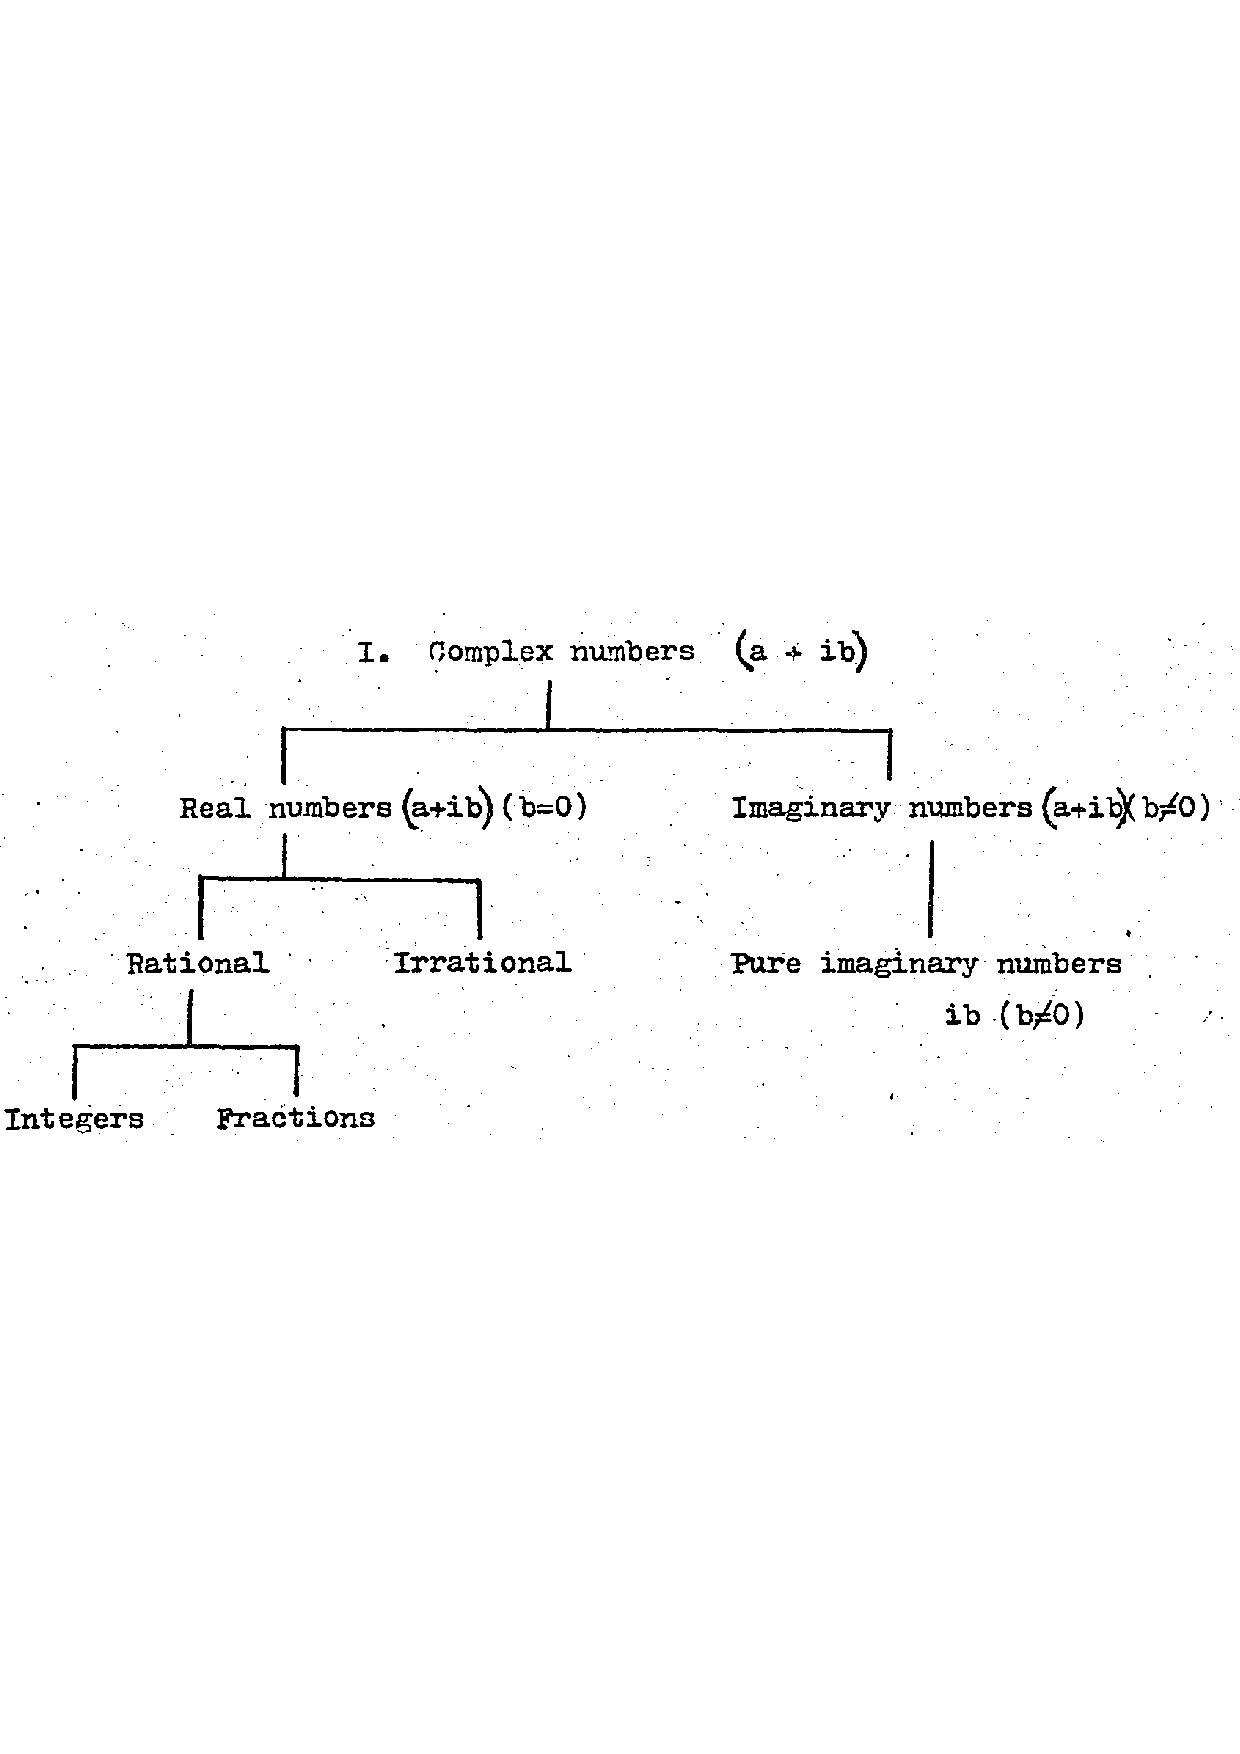
\includegraphics[width=0.9\textwidth]{images/SD-1-1p15A}
%	\caption{Classification of complex numbers}
%	\label{fig:classificationOfComplexNumbersA}
%\end{figure}

%\begin{center}
%\begin{tabular}{cc}
%\end{tabular}
%\end{center}

%\begin{exmp}
%\begin{hSolution}
%\end{hSolution}
%\end{exmp}

%\begin{hEnumerateAlpha}
%\end{hEnumerateAlpha}

%\begin{hEnumerateRoman}
%\end{hEnumerateRoman}

%$
%\begin{bmatrix}
%\end{bmatrix}
%$

%\frac{aaaa}{bbb}
%\frac{a_{n}}{b_{n}}
%\left( aaaa \right)
%\Longrightarrow

%\begin{multicols}{2}
%	bb
%\columnbreak
%	aa
%\end{multicols}
